\section{Background and Motivation}
\label{sec:background}


An LLM service follows a client-server architecture: the client submits a sequence of text as a request to the server; the server hosts the LLM on GPUs, runs inference over the request, and responds (or streams) the generation back to the client. As explained in \S\ref{sec:introduction}, due to the unique prefill-decoding process, LLM service may impose aggressive service-level objectives (SLOs) on both TTFT and TPOT, varying with the application's needs. The serving system must meet both SLOs while minimizing the cost associated with expensive GPUs. In other words, we want the serving system to maximize the requests served per second adhering to the SLO attainment goal for each GPU provisioned -- \emph{maximizing per-GPU goodput}.
Next, we detail the LLM inference computation (\S\ref{sec:llm-inference}) and discuss existing optimizations for LLM serving (\S\ref{sec:llm-serving}).

\subsection{LLM Inference}
\label{sec:llm-inference}

Modern LLMs~\cite{openai2023gpt4,touvron2023llama} predict the next token given an input sequence. This prediction involves computing a hidden representation for each token within the sequence. An LLM can take a variable number of input tokens and compute their hidden representations in parallel, and its computation workload increases superlinearly with the number of tokens processed in parallel. Regardless of the input token count, the computation demands substantial I/O to move LLM weights and intermediate states from the GPU's HBM to SRAM. This process is consistent across varying input sizes.

The prefill step deals with a new sequence, often comprising many tokens, and processes these tokens concurrently. Unlike prefill, each decoding step only processes one new token generated by the previous step.
This leads to significant computational differences between the two phases.
When dealing with user prompts that are not brief, the prefill step tends to be compute-bound. For instance, for a 13B LLM, computing the prefill of a 512-token sequence makes an A100 near compute-bound (see \S\ref{subsec:analysis_prefill}). In contrast, despite processing only one new token per step, the decoding phase incurs a similar level of I/O to the prefill phase, making it constrained by the GPU's memory bandwidth.

During both phases, intermediate states, known as KV caches~\cite{vllm}, are generated at each token position, which are needed again in later decoding steps. To avoid recomputing them, they are saved in GPU memory. 
Because of the shared use of LLM weights and KV caches in memory, most LLM inference engines opt to colocate the prefill and decoding phases on GPUs, despite their distinct computational characteristics.

\subsection{LLM Serving Optimization}
\label{sec:llm-serving}
In real-time online serving, multiple requests come and must be served within SLOs. Batching and parallelizing their computation is key for achieving low latency, high throughput, and high utilization of GPUs. 

\parabf{Batching.} 
Current serving systems~\cite{yu2022orca,vllm, agrawal2023sarathi} utilize a batching technique known as \emph{continuous batching}. This method batches the prefill of new requests with the decoding of ongoing ones. It boosts the GPU utilization and maximizes the overall system throughput -- tokens generated per second across all users and requests.
However, as mentioned in \S\ref{sec:introduction} and elaborated later in \S\ref{sec:problem-opportunity}, this approach leads to trade-offs between TTFT and TPOT.
An advanced variant of continuous batching~\cite{agrawal2023sarathi} attempts to balance TTFT and TPOT by segmenting long prefill into chunks and attaching decoding jobs with a chunked prefill  --  but essentially, it trades TTFT for TPOT and cannot eliminate the interference (\S\ref{sec:problem-opportunity}).
In summary, batching prefill and decoding invariably leads to compromises in either TTFT or TPOT.

\parabf{Model parallelism.} In LLM serving, model parallelism is generally divided as intra- and inter-operator parallelisms~\cite{li2023alpaserve,alpa,shoeybi2020megatronlm}. Both can be used to support larger models but may impact serving performance differently. 
Intra-operator parallelism partitions computationally intensive operators, such as matrix multiplications, across multiple GPUs, accelerating computation but causing substantial communication. 
It reduces the execution time\footnote{we emphasize ``execution time'' instead of latency here because latency comprises both execution time and queuing delay.}, hence latency, particularly for TTFT of the prefill phase, but requires high bandwidth connectivity between GPUs (e.g., NVLINK).
Inter-operator parallelism organizes LLM layers into stages, each running on a GPU to form pipelines. It moderately increases execution time due to inter-stage communication, but linearly scales the system's rate capacity with each added GPU.
In this paper, we reveal an additional benefit of model parallelism: reduced queuing delay of both prefill and decoding phases, steaming from shorter execution time. We delve into this further in \S\ref{sec:tradeoff}.
Besides model parallelism, replicating a model instance, irrespective of its model parallelism configurations, linearly scales the system's rate capacity.

These parallelism strategies create a complex space of optimization that requires careful trade-offs based on the application's latency requirements.

\subsection{Problems and Opportunities}
\label{sec:problem-opportunity}
Colocating and batching the prefill and decoding computation to maximize the overall system throughput, as in existing systems, is cost-effective for service providers. However, in the presence of SLOs, present approaches struggle to maintain both high service quality and low cost due to the issues discussed below.

\begin{figure}[t]
    \centering
    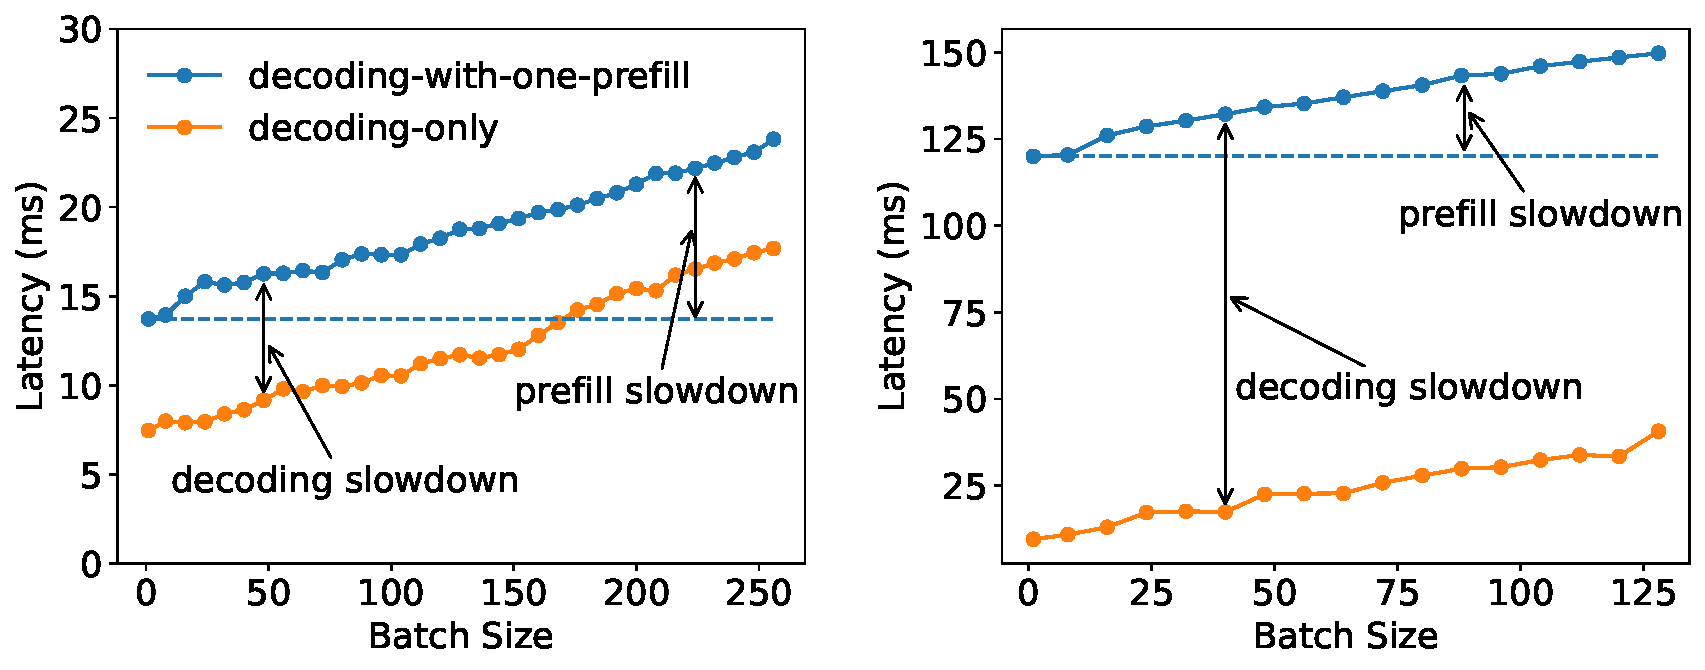
\includegraphics[width=\columnwidth]{figures/prefill-decoding-interference.pdf}
    (a) Input length = 128 \hspace{11mm} (b) Input length = 1024
    \vspace{-2mm}
    \caption{Batch execution time when serving a 13B LLM as batch size increases. Compared between a decoding-only batch and the batch adding one more prefill job.}
    \vspace{-6mm}
    \label{fig:interference}
\end{figure}

\parabf{Prefill-decoding interference.} As Figure~\ref{fig:interference} shows, adding a single prefill job to a batch of decoding requests significantly slows down both processes, leading to a marked increase in TTFT and TPOT. 
% Even worse, as the input length increases, the slowing down of decoding by prefill becomes more pronounced due to the long execution time of prefill job. 
Specifically, the decoding tasks in the batch must wait for lengthier prefill jobs to complete, thus extending TPOT; the slowdown intensifies with a longer prefill, shown in Figure~\ref{fig:interference}\textcolor{green!80!black}{(b)}.
Adding decoding jobs to prefill also increases the time to complete the prefill task, particularly when the GPU is already at capacity (Figure~\ref{fig:interference} blue curves). 

One attempt to mitigate this interference is called \textit{chunked-prefill with piggyback}~\cite{agrawal2023sarathi, deepspeed_mii}. It proposes to split the long prefill into chunks and batch a prefill chunk with a few decoding jobs (a.k.a. piggybacking). This technique alleviates the slowdown of the decoding job caused by the long prefill job, but it does not eliminate it. Additionally, it results in an extra overhead for the prefill job which cannot be easily mitigated by adjusting the chunk size. First, if the chunk size is set much lower than the inflection point that can saturate the GPU, then the prefill job will have a longer execution time since it competes with the decoding job in the same batch and cannot solely utilize the GPU resources. Second, if we increase the chunk size to nearly saturate the GPU, the chance of piggybacking will diminish since the remaining slots for decode tokens are limited. Also, chunked-prefill causes significantly more memory access for the prefill jobs. This is because the KV cache of all previous chunks have to be loaded from HBM to SRAM repeatedly to compute each subsequent chunk. Concretely, if a prefill job is split into $N$ equal chunks, we need to load $N + (N-1) + ... + 1 = O(N^2)$ chunks of KV Cache in total, compared to O(N) in the non-chunked case. This overhead will increase as the context length becomes longer.

\parabf{Ineffective scheduling.} Unbatching prefill and decoding jobs and scheduling them sequentially does not mitigate the interference. Decoding jobs may experience longer queuing delays due to waiting for ongoing prefill jobs on GPUs. Moreover, batches dedicated to decoding often lead to GPU underutilization. Prioritizing tasks in either phase adversely affects the latency of the other, rendering priority scheduling ineffective.

\parabf{Resource and parallelism coupling.} Colocating prefill and decoding phases on the same GPUs unavoidably share their resource and parallelism settings. However, each phase has its unique computational characteristic and latency requirement that calls for more heterogeneous resource allocation. 
For example, the prefill phase tends to be compute-bound and benefits from more intra-op parallelism to reduce execution time to meet the tight SLO on TTFT. By contrast, the optimal parallelism configuration of the decoding phase depends on the running batch size.
In existing systems, due to coupling, resource allocation and parallelism plans are tailored to satisfy the \emph{more demanding} of TTFT and TPOT, which may not be ideal for the other. This often leads to resource over-provisioning to meet both SLOs. 

\parabf{Opportunities.} To address these issues, we propose to disaggregate the prefill and decoding phases. We use the term \textit{instance} to denote a unit of resources that manages exactly one complete copy of model weights. One instance can correspond to many GPUs when model parallelism is applied.
Note that when we disaggregate the two phases to different GPUs, each phase manages its copy of the model weights, resulting in \emph{prefill instances} and \emph{decoding instances}. A prefill instance, upon receiving a request, performs only the prefill computation for this request to generate the first output token. It then sends the intermediate results (mainly KV caches) to a decoding instance, which is responsible for subsequent decoding steps. 
Because decoding computation often has low GPU utilization, we may allocate multiple prefill instances per decoding instance. This allows batching more decoding jobs to achieve higher GPU utilization.

Disaggregating prefill and decoding naturally resolves the interference between the two phases and enables each to focus on its optimization target -- TTFT or TPOT. Each type of instance can employ different resources and parallelism strategies to meet a variety of latency requirements. 
By adjusting the number of GPUs and parallelisms provided to the two types of instances, we can maximize the per-device goodput of the overall system, avoiding over-provisioning, eventually translating to reduced cost-per-query adhering to service quality. Next, we develop ways to find out the best resource allocation and parallelism plan for each phase.